\documentclass{article}[18pt]
\usepackage[utf8]{inputenc}
\usepackage[margin=0.7in]{geometry}
\usepackage{parselines} 
\usepackage{amsmath}
\usepackage{amssymb}
\usepackage{relsize}
\usepackage{titlesec}
\usepackage{pgfplots}
\usepackage{graphicx}
\usepackage[english]{babel}
\usepackage{fancyhdr}
\usepackage{gensymb}
\usepackage{tikz}
\usetikzlibrary{positioning}
\pgfplotsset{width=10cm,compat=1.9}

\titlespacing\section{0pt}{14pt plus 4pt minus 2pt}{0pt plus 2pt minus 2pt}
\newlength\tindent
\setlength{\tindent}{\parindent}
\setlength{\parindent}{0pt}
\renewcommand{\indent}{\hspace*{\tindent}}

\pagestyle{fancy}
\fancyhf{}
\rhead{Sam Robbins 13SE}
\lhead{A Level Maths - M2}
\rfoot{Page \thepage}


\begin{document}
\begin{center}
\underline{\huge Kinematics}
\end{center}
\begin{obeylines}
\section{Horizontal Projections}
For a \textbf{constant speed} use \textbf{$Speed=\dfrac{Distance}{Time}$}

For a \textbf{constant acceleration} use \textbf{SUVAT}

For all projections:
\begin{itemize}
\item Assume air resistance to be zero
\item Resolve horizontal and vertical motion
\item Horizontal - Constant speed
\item Vertical - Constant acceleration

\end{itemize}

\section{Angular projections}
The same as horizontal projections but the initial vertical velocity isn't zero.
Example:
A particle is projected at a speed of $49ms^{-1}$ at an angle of $45 \degree$ above the horizontal.
\textit{What is the time taken for the particle to reach its maximum height?}
\begin{itemize}
\item u=$49\sin45$
\item v=0
\item a=-g
\item t=?
\end{itemize}
$0=49\sin45-gt$
$t=\dfrac{49\sin45}{g}=\dfrac{5\sqrt{2}}{2}\approx3.54$
\textit{What is the maximum height reached?}
\begin{itemize}
\item u=$49\sin45$
\item v=0
\item a=-g
\item s=?
\end{itemize}
$v^2=u^2+2as$
0=$(49\sin45)^2-2gs$
$S=\dfrac{(49\sin45)^2}{2g}=61.3$
\textit{What is the time of the flight?}
\begin{itemize}
\item u=$49\sin45$
\item a=-g
\item S=0
\item t=?
\end{itemize}
$S=ut+\dfrac{1}{2}at^2$
$ $
$0=(49\sin45)t-\dfrac{1}{2}gt^2$
0=$t(49\sin45-\dfrac{gt}{2}$
$t=0$
$49\sin45=\dfrac{gt}{2}$
$t=\dfrac{2\times49\sin45}{g}=7.07$
\textit{What is the horizontal range of the particle?}
\begin{itemize}
\item t=7.07
\item Speed=$49\cos45$
\end{itemize}
$S=45\cos45\times7.07=245$
\end{obeylines}
\section{Displacement, velocity and acceleration}
$v=\dfrac{dx}{dt}$\\
\\
$a=\dfrac{dv}{dt}$\\
\\
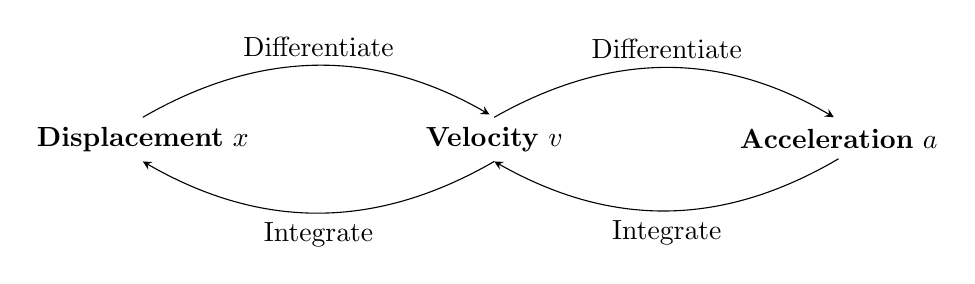
\begin{tikzpicture}
  \node (disp) {\textbf{Displacement} $x$};
  \node[right=2cm of disp] (vel) {\textbf{Velocity} $v$};
  \node[right=2cm of vel] (acc) {\textbf{Acceleration} $a$};
  \draw[-stealth,shorten >= 2pt] (disp.north) to[bend left] node[midway,above] {Differentiate} (vel.north);
  \draw[-stealth] (vel.south) to[bend left] node[midway,below] {Integrate} (disp.south);
  \draw[-stealth,shorten >= 2pt] (vel.north) to[bend left] node[midway,above] {Differentiate} (acc.north);
    \draw[-stealth] (acc.south) to[bend left] node[midway,below] {Integrate} (vel.south);
\end{tikzpicture}
\newpage
\begin{center}
\underline{\huge Kinematics Example - Problems with calculus}
\end{center}
\textit{A particle P moves along the x-axis in a straight line so that, at time t seconds, the velocity of P is $v \ \text{ms}^{-1}$, where}\\
\\
$
  v=\left\{
  \begin{array}{@{}ll@{}}
    10t-2t^2, & \text{for}\ 0\leqslant t \leqslant 6  \\
    -\dfrac{432}{t^2}, & t>6
  \end{array}\right.
$\\
\\
\\
\textit{At $t = 0$, P is at the origin O. Find the displacement of P from O when}\\
\\
$\mathit{t = 6}$\\
\\
\textbf{Integrate velocity}\\
\\
\textcolor{red}{$\mathlarger{x=\int v \ dt}$}\\
\\
$x=\int 10t-2t^2 \ dt= 5t^2-\frac{2}{3}t^3+c$\\
\\
\\
\textbf{Substitute in the value of t}\\
\\
$t=6$\\
\\
$x=5\times6^2-\frac{2}{3}\times6^3=36m$\\
\\
\\
$\mathit{t = 10}$
\\
\textbf{Integrate velocity for the second half of the journey}\\
\\
$x=\mathlarger{\int-\dfrac{432}{t^2} \ dt=\int-432t^{-2} \ dt=\dfrac{-432t^{-1}}{-1}+k=\dfrac{432}{t}+k}$\\
\\
\textbf{Find value of k by using known distance at t=6}\\
\\
$t=6 \ \ x=36$\\
\\
$36=\dfrac{432}{6}+k$\\
\\
$k=36-72=-36$\\
\\
\textbf{Find distance using value of k and t}\\
\\
$t=10$\\
\\
$x=\dfrac{432}{10}-36=7.2\text{m}$




\end{document}